%
%
%

\chapter{Complex Numbers and Logs Review}

\section{Problem Statement and Learning Objectives}
This appendix contains quizes to determine if you need to review complex numbers and/or logarithms, as well as some material to support that review.

Be able to
\begin{itemize}
    \item Pass the Complex Number quiz below.
    \item Pass the Logarithms quiz below. 
\end{itemize}

%%%%%%%%%%%%%%%%%%%%%%%%%%%%%%%%%%%%%%%%%%%%%%%%%%%%%%%%%%%%%%%%%%%%%%%%%%%%%%%%%%%%%%%%%%%%%%%%%%%%%%%%%%%%%%%%%%%%%%
\section{Complex Number Quiz}\label{ComplexNumberReview}
Take this quiz then check your answers on Page \pageref{CN_answers}.  Use only the following functions on your calculator (or fewer as instructed):

\[
* \quad \div + \quad - \quad \sqrt{x}
\]


It should be {\bf easy for you to get exact answers}.  If not, then you need to review the concepts in this quiz and section \ref{cnconcepts}.   Some Kahn Academy videos are pre-linked in Section \ref{KahnV}.


\begin{enumerate}

\item  What is $\sqrt{-16}$ ?

\item  Evaluate
\[
X = \frac{-b + \sqrt{4ac}}{2a}
\]
for the following values:
\begin{quotation}
\begin{tabular} {c|c|c}
a&b&c  \\ \hline
1&2&3 \\
1&-4&29\\
2&28&1156
\end{tabular}
\end{quotation}


\item  Evaluate
\[
(6+j16) + (-7-j6) =
\]
\[
(27-j0.75) - (1.6+j0.27) =
\]


\item  Evaluate  $M\times N$ where

\begin{quotation}
\begin{tabular} {c|c}
M&N \\ \hline
$(2+6j)$	&	$(1+3j)$   	\\
$(1.7-0.6j)$    &	$(3.2+0.4j)$	\\
\end{tabular}
\end{quotation}


\item  Plot the following points on the complex plane:
\[
a = -3+1.5j \qquad b = 2-j \qquad c = j
\]


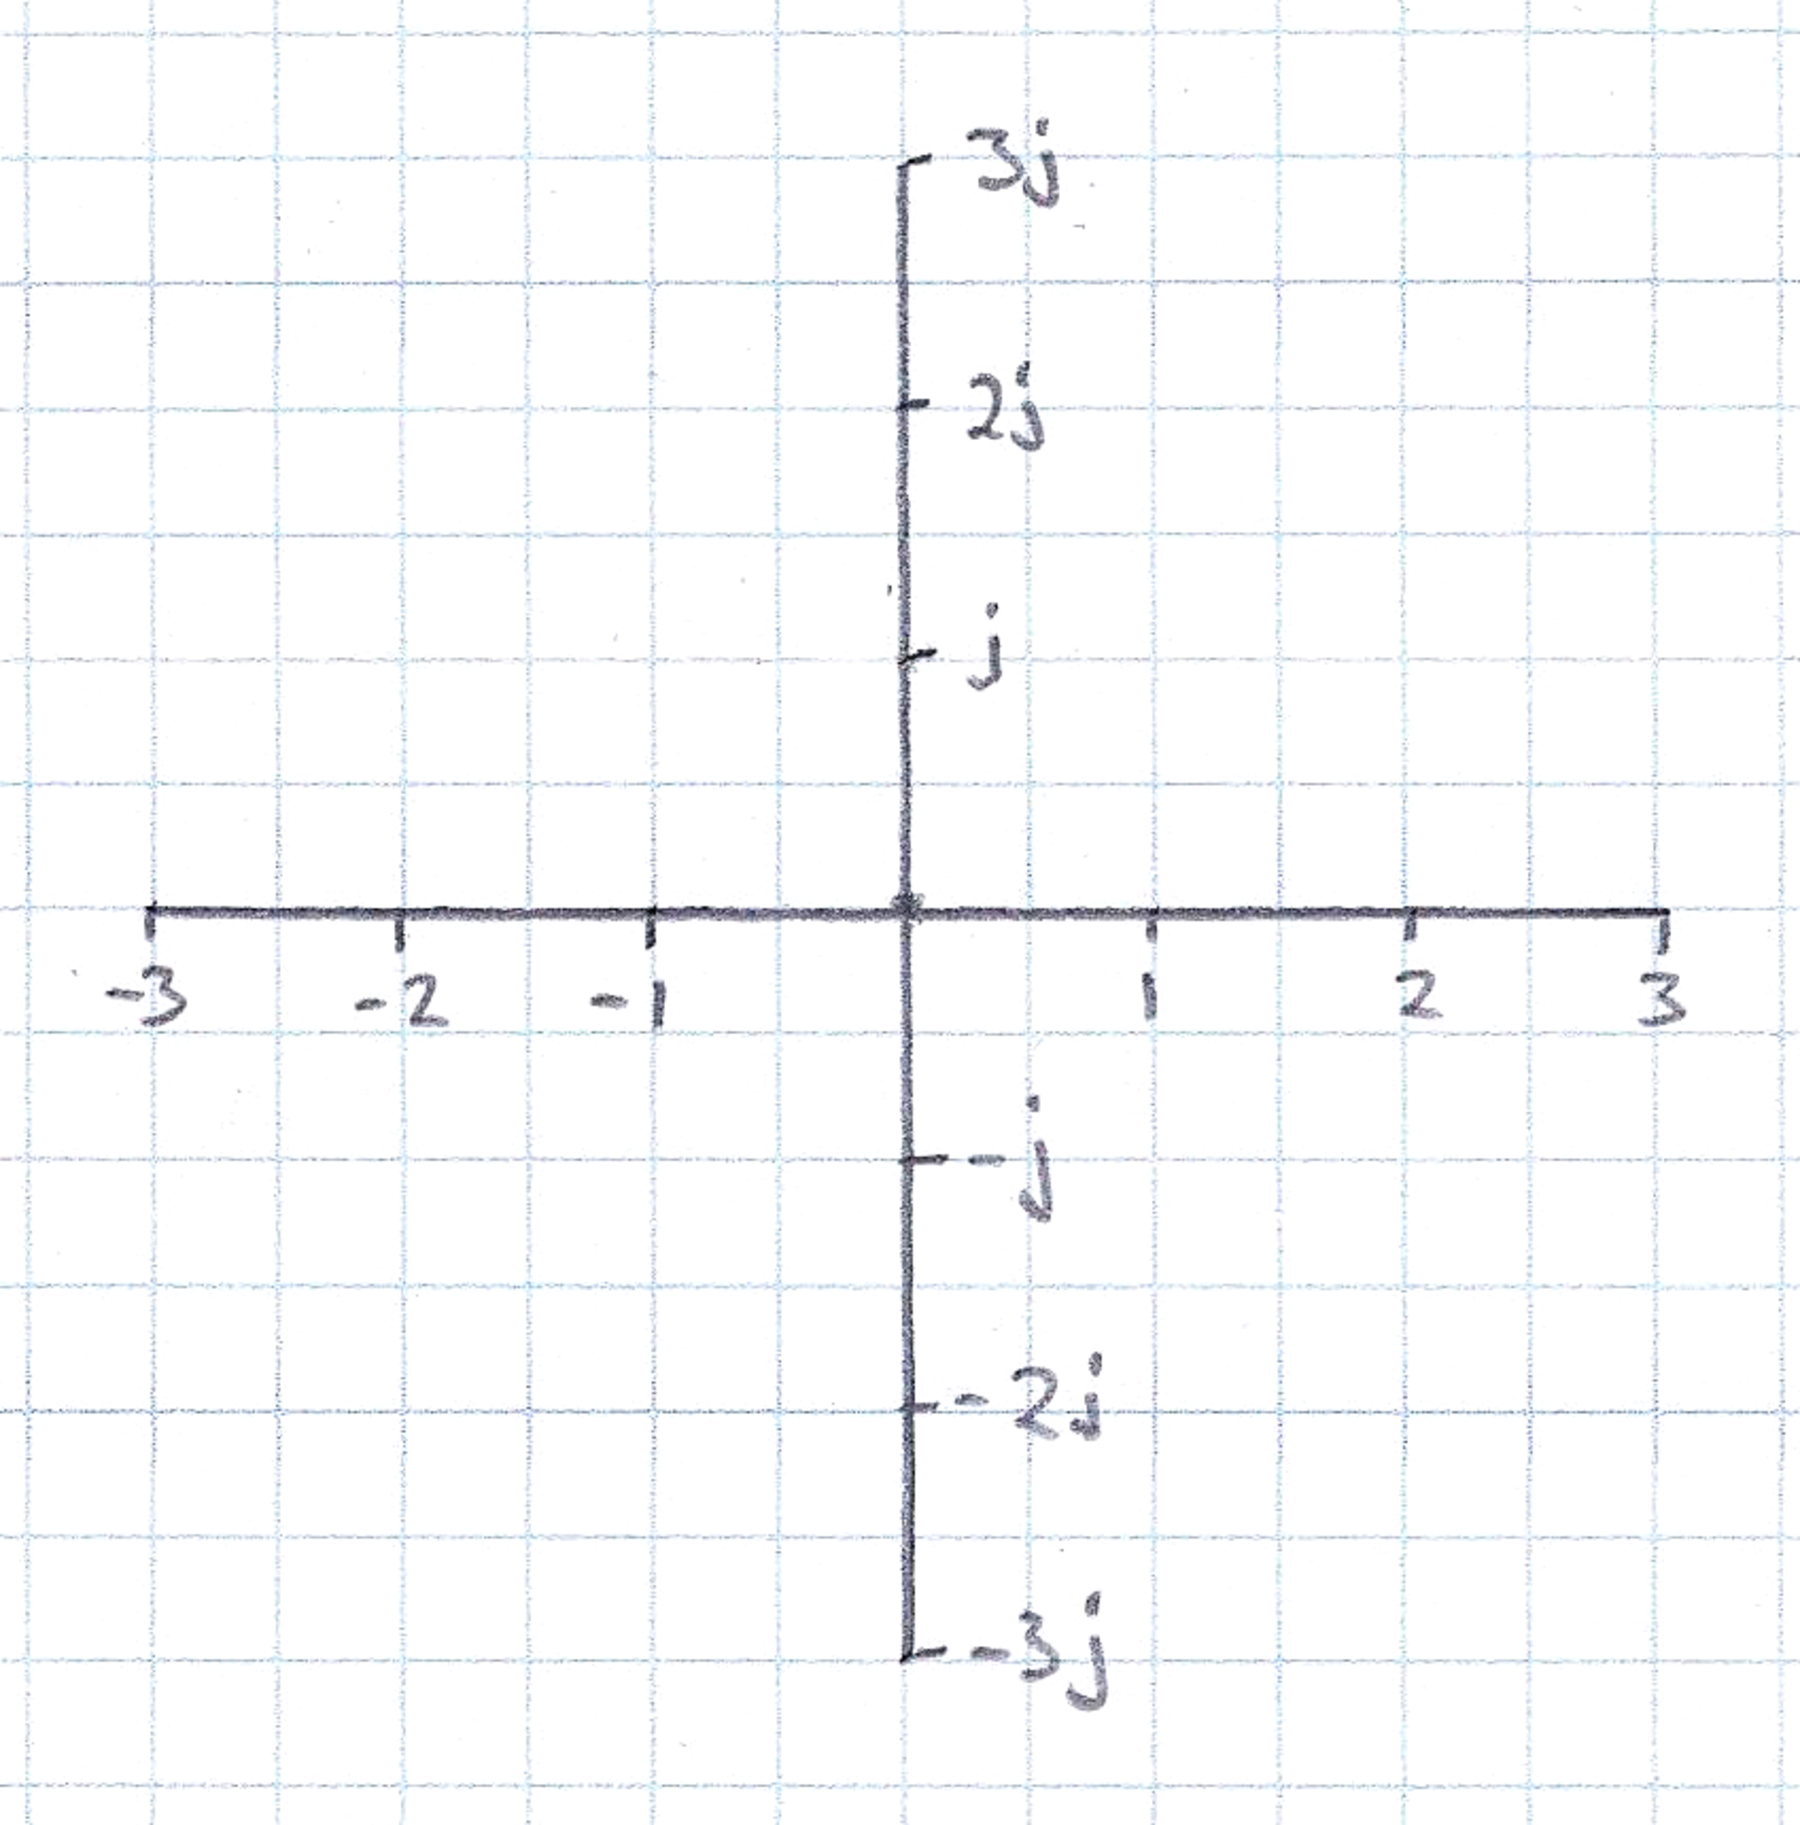
\includegraphics[width=6cm]{figsapdx/00926a.png}



\item  Convert $X_1=(4+3j)$ to polar (magnitude-angle) form


\item  Convert $X_2=(-16+3.7j)$ to polar (magnitude-angle) form


\item  Represent $X_3 = (-1+6j)$ in exponential form

\item  For
\[
a = 3e^{j\pi/4} \qquad b = 2\angle{45^\circ}
\]
Convert them to ``$a+bj$'' form and multiply $a*b$ without using a calculator.

\end{enumerate}








\section{Complex Number Concepts required for EE447}\label{cnconcepts}
\begin{itemize}
  \item $j = \sqrt{-1}$
  \item complex number is the sum of a real part, $\sigma$ + an imaginary part $j\omega$ (where $\omega$ is a real number to be multiplied by $j$.)
  \item   The {\it magnitude} of a complex number is the Pythagorean sum of the real and imaginary parts:
  If $x= a+jb$ is a complex number, then the magnitude is
  \[
  |x| = \sqrt{a^2+b^2}
  \]
  \item To add together two complex numbers, add their real and imaginary parts separately.
  \[
  x = a+bj \qquad y = c+dj
  \]
  \[
  x + y = (a+c) + j(b+d)
  \]
  \item To multiply two complex numbers, multiply them together like two first order polynomials in $j$ (using the definitions above)
  \[
  x*y = (a+bj)*(c+dj) = ac+adj + bcj+bdj^2
  \]
  since $j^2=-1$ we have
  \[
  x*y = (ac-bd)+(ad+bc)j
  \]

  \item Complex numbers describe a point in the {\it complex plane}.  The $X$ axis of the complex plain is the real part of the complex number and the $Y$ axis is the imaginary part.

  \item To plot the point $a+jb$ on the complex plane, plot a point at $X = a, \: Y = b$.

  \item The magnitude of a complex number is the distance from the origin to its point on the complex plane.

  \item The {\it angle} of a complex number is the angle formed from the positive real axis ($X>0$) and the line between the origin and the point.

  \item There is an \href{http://en.wikipedia.org/wiki/Euler\%27s_formula}{exponential form} of any complex number:
  \[
  e^{j\theta} = \cos(\theta) + j\sin(\theta)
  \]
  \item To convert a complex number to exponential form we invert the previous equation:
  \[
  a+bj = |a+bj| e^{j\tan^{-1}(b/a)}
  \]

  \item The $\tan^{-1}()$ function traditionally limits us to quadrants I and IV of the complex plain.    More generally we can use the 4-quadrant 2-argument arctan function \href{http://en.wikipedia.org/wiki/Atan2}{({\tt atan2(b,a)}) }.

  \item A consequence of multiplication of complex numbers and the exponential represenation of complex numbers is that when we multiply two complex numbers:
     \begin{quotation} {\it ``angles add and magnitudes multiply''}
     \end{quotation}
   if $A,B,C$ are complex numbers and $C = A * B$
   \[
    \angle{C} = \angle{A}+\angle{B}  \qquad   |C| = |A|*|B|
   \]


\end{itemize}

\section{Kahn Academy Videos}\label{KahnV}

\href{https://www.khanacademy.org/math/algebra/complex-numbers/complex_numbers/v/complex-numbers}{complex numbers}

\href{https://www.khanacademy.org/math/trigonometry/imaginary_complex_precalc/complex_analysis/v/exponential-form-to-find-complex-roots}{exponential form of complex numbers}








%%%%%%%%%%%%%%%%%%%%%%%%%%%%%%%%%%%%%%%%%%%%%%%%%%%%%%%%%%%%%%%%%%%%%%%%%%%%%%%%%%%%%%%%%%%%%%%%%%%%%%%%%%%%%%%%%%%%%%%%
\section{Logs}\label{LogReview}

Although logarithms are pretty basic material, experience shows that many students are rusty on logs at the start of EE447.
We all know how to press the LOG button on a calculator, the problems come in some of the concepts.


\section{Logarithms Quiz}

Take this quiz then check your answers on Page \pageref{Log_answers}.  If the problem is numerical, you may use only the following functions on your calculator (or fewer as instructed):

\[
* \quad \div \quad + \quad -
\]


It should be {\bf easy for you to get exact answers}.  If not, then you need to review the concepts


\begin{enumerate}

\item  Find the log of $A*B$

\item  Find the log of $(a^2) * \sqrt(b)$

\item  Find the log (base 10) of $\frac{1,000,000}{R}$

\item  Find the natural log of $e^{27.4}$

\item  Find the base 10 log of $e^{27.4}$


\end{enumerate}






%%%%%%%%%%%%%%%%%%%%%%%%%%%%%%%%%%%%%%%%%%%%%%%%%%%%%%%%%%%%%%%%%%%%%%%%%%%%%%%%%%%%%%%%%%
\newpage
\section{Complex Number Quiz Answers}\label{CN_answers}

\begin{enumerate}
\item 4j

\item $-1\pm j\sqrt{2} \qquad  2\pm j5 \qquad -7\pm j23  $

\item $-1+j10 \qquad 1.1-j1.02$

\item $-16+12j \qquad 5.68-1.24j$

\item graphing points $a,b,c$:

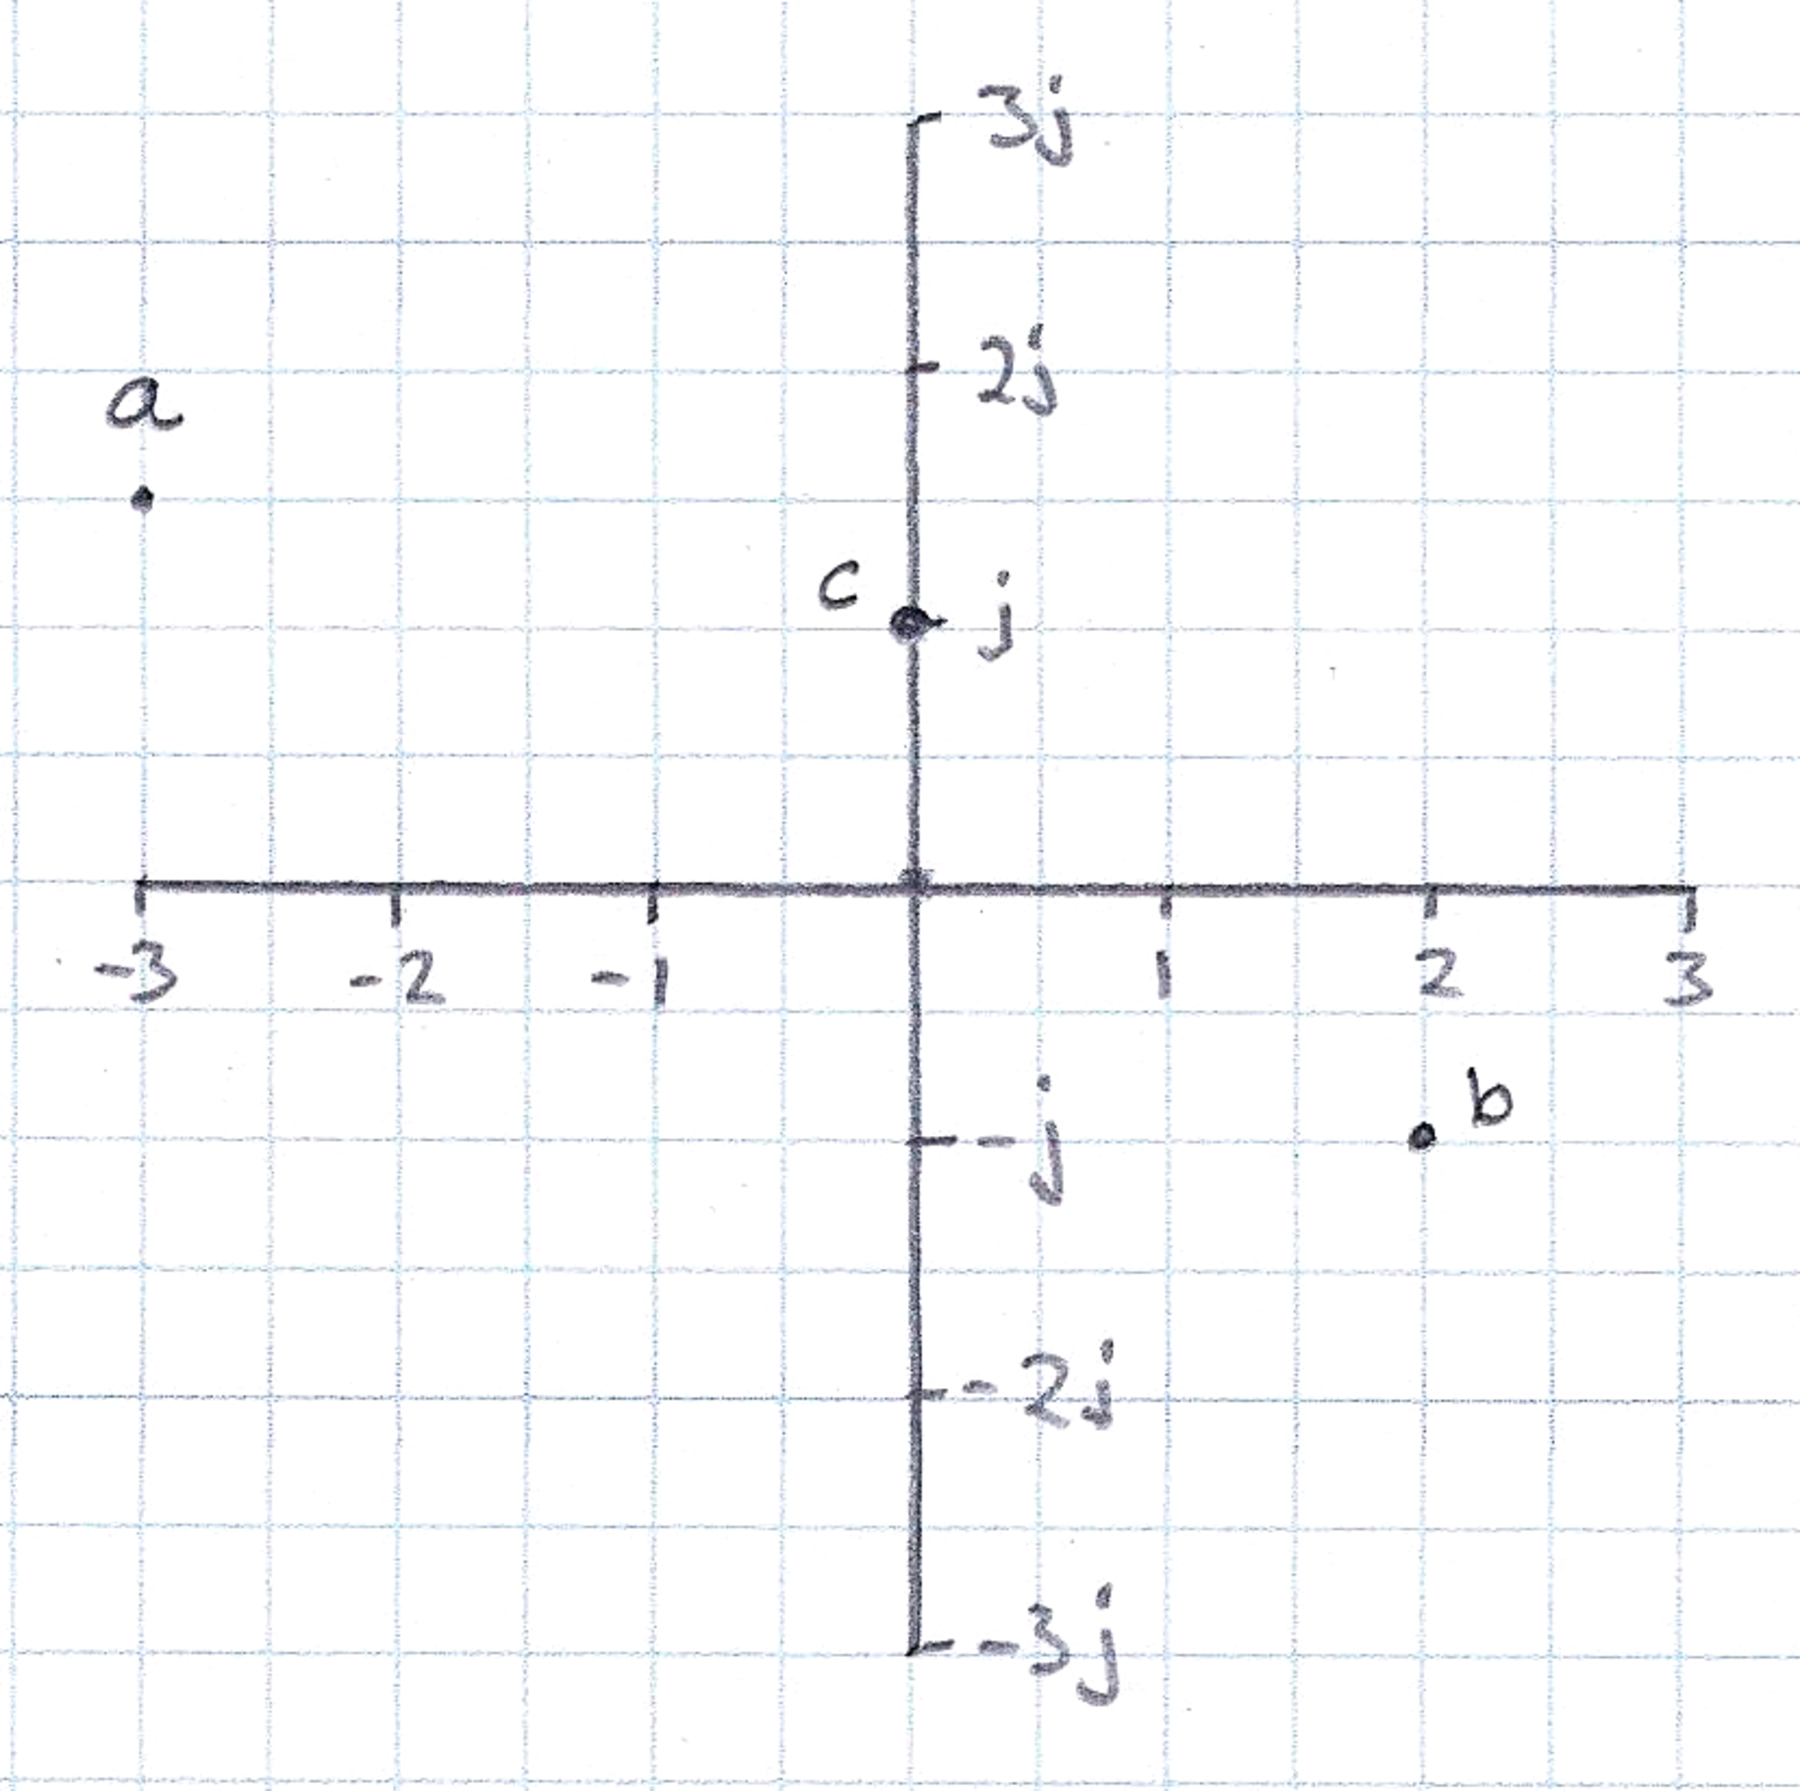
\includegraphics[width=6cm]{figsapdx/00927a.png}

\item $|X_1| = 5 \qquad \angle X_1 = \tan^{-1}(4/3) = 53.1^\circ$

\item $|X_2| = 16.42 \qquad \angle{X_2} = 167^\circ$

\item $X_3 = 6.08e^{j1.74}$ (note radians must be used in the exponential)

\item $|a| = 3, \; |b| = 2$,  $\angle a = 45^\circ,\; \angle b = 45^\circ$  by inspection.
\[
a = 3*0.707 + j3*0.707 = .2121+j.2121 \qquad b = 2*.707 + j2*.707 = .1414+j.1414
\]
using {\it angles add, magnitudes multiply}, $a*b = 3*2e^{j\frac{\pi}{2}} = 6e^j = 6j$

\end{enumerate}


%%%%%%%%%%%%%%%%%%%%%%%%%%%%%%%%%%%%%

\section{Log Quiz Answers}\label{Log_answers}


\begin{enumerate}

\item $\log(A) + \log(B)$

\item $2\log(a)+\frac{\log(b)}{2}$

\item $6-\log(R)$

\item $27.4$

\item $27.4/\ln(10)$

\end{enumerate}



% \section{Summary of Notation}

